\documentclass[10pt,twocolumn]{article}
\usepackage[letterpaper,margin=0.75in,columnsep=0.25in]{geometry}
\usepackage[T1]{fontenc}
\usepackage{amsmath,amsthm}
\usepackage{newtxtext,newtxmath}
\usepackage[authoryear,round]{natbib}
\usepackage{graphicx,booktabs,microtype,xcolor}
\usepackage{algorithm,algpseudocode}
\usepackage[font=small,labelfont=bf,skip=4pt]{caption}
\usepackage{titlesec,enumitem}
\usepackage[colorlinks=true,linkcolor=blue!45!black,citecolor=blue!45!black,urlcolor=blue!45!black]{hyperref}
\usepackage{xurl}
\titleformat{\section}{\normalfont\large\bfseries}{\thesection}{.6em}{}
\titleformat{\subsection}{\normalfont\normalsize\bfseries}{\thesubsection}{.5em}{}
\titlespacing*{\section}{0pt}{9pt}{4pt}
\titlespacing*{\subsection}{0pt}{7pt}{3pt}
\setlength{\textfloatsep}{9pt plus 2pt minus 2pt}
\setlength{\floatsep}{8pt plus 2pt minus 2pt}
\setlength{\dbltextfloatsep}{10pt plus 2pt minus 2pt}
\theoremstyle{plain}\newtheorem{proposition}{Proposition}
\theoremstyle{definition}\newtheorem{corollary}{Corollary}
\newcommand{\ConfTasks}{48}
\newcommand{\ConfOutputs}{68}
\newcommand{\ConfSolved}{14}
\newcommand{\ConfOracle}{18}
\newcommand{\ConfMissed}{4}
\newcommand{\ConfNoCorrect}{50}
\newcommand{\ConfEmpty}{18}
\newcommand{\Unreach}{13}
\newcommand{\UnreachEmpty}{12}
\newcommand{\Reach}{55}
\newcommand{\ReachEmpty}{6}
\newcommand{\TightN}{11}
\newcommand{\TightEmpty}{4}
\newcommand{\TightOracle}{1}
\newcommand{\StepMs}{103}
\newcommand{\StepLo}{101}
\newcommand{\StepHi}{112}
\newcommand{\StepTasks}{6}
\newcommand{\EvalOutputs}{172}
\newcommand{\EvalTasks}{120}
\newcommand{\EvalUnreach}{48}
\newcommand{\EvalUnreachPct}{28}
\newcommand{\EvalTasksUnreach}{32}
\newcommand{\EvalOver}{74}
\newcommand{\EvalOverPct}{43}
\newcommand{\ExtEligible}{18}
\newcommand{\CloneTrials}{213}
\newcommand{\CloneRef}{55}
\newcommand{\CloneAnchor}{39}
\newcommand{\TrainReach}{2}
\newcommand{\TrainN}{9}
\newcommand{\SFourBase}{4}
\newcommand{\SFourRepair}{5}
\newcommand{\SFourRiskOnly}{5}
\newcommand{\SFourOracle}{7}
\newcommand{\SFourN}{35}
\newcommand{\SFourTasks}{24}
\newcommand{\SFourRepairs}{76}

\newcommand{\PilotN}{9}
\newcommand{\PilotEmptyCtl}{7}
\newcommand{\PilotEmptyLA}{1}
\newcommand{\PilotCovCtl}{1}
\newcommand{\PilotCovLA}{3}
\newcommand{\PilotSolvedCtl}{0}
\newcommand{\PilotSolvedLA}{2}
\newcommand{\PilotLosses}{0}
\newcommand{\PilotEq}{12}
\newcommand{\PilotEqN}{12}
\newcommand{\PilotMsParent}{103.1}
\newcommand{\PilotMsIter}{99.9}
\newcommand{\PilotRatio}{0.999}
\newcommand{\PilotMaxTokens}{930}
\newcommand{\PilotFinCtl}{20}
\newcommand{\PilotFinLA}{58}
\newcommand{\PilotGridsCtl}{10}
\newcommand{\PilotGridsLA}{32}
\newcommand{\ScoreBZero}{25.28}
\newcommand{\ScoreSOne}{22.78}
\newcommand{\ScoreSTwo}{23.61}
\newcommand{\ScoreLOne}{26.94}
\newcommand{\ConfN}{48}
\newcommand{\ConfT}{32}
\newcommand{\ConfSolvedCtl}{5}
\newcommand{\ConfSolvedLA}{13}
\newcommand{\ConfGains}{8}
\newcommand{\ConfLosses}{0}
\newcommand{\ConfEmptyCtl}{28}
\newcommand{\ConfEmptyLA}{5}
\newcommand{\ConfCovCtl}{5}
\newcommand{\ConfCovLA}{13}
\newcommand{\ConfLo}{6.0}
\newcommand{\ConfHi}{29.8}
\newcommand{\ConfRatio}{0.996}
\newcommand{\ConfDelta}{16.7}

\newif\ifpilot\pilottrue
\newif\ifconf\conftrue


\begin{document}
\twocolumn[{
\begin{center}
{\LARGE\bfseries Out of Time: Where Test-Time-Trained\\[3pt] ARC-AGI-2 Solvers Lose Their Answers\par}
\vspace{9pt}
{\normalsize Jingtao Huang \qquad Kaggle: \texttt{huangjt66}}\\[3pt]
{\small ARC Prize 2026 Paper Track \quad$\cdot$\quad linked ARC-AGI-2 entries in Table~\ref{tab:leaderboard}}
\vspace{9pt}
\end{center}
\begin{abstract}
\noindent Before a model can be right about an ARC-AGI-2 task, it has to finish writing the answer. We show that this obvious requirement quietly limits the test-time-trained language-model solvers that lead the Kaggle competition. Replaying the frozen candidate pools of a working entry on \ConfOutputs{} held-out outputs, eight different selectors solve the same \ConfSolved{}, and only \ConfOracle{} pools contain the answer at all: generation, not selection, sets the ceiling. A one-line bound explains much of the gap. An $h\times w$ grid takes $hw+h$ sequential decoding steps, and the common practice of splitting a fixed budget evenly across view batches can leave no batch enough time for a long answer. None of the \Unreach{} outputs that violate the bound has a correct candidate, and under the same budget \EvalUnreachPct\% of all ARC-AGI-2 public evaluation outputs cannot be decoded at all. We introduce \emph{length-aware decoding}: an exact, recursion-free reimplementation of the solver's depth-first search, and a schedule that lets a view finish its first greedy path before the next view begins. With the same adapted model and the same 180 seconds, it reduces empty candidate pools from \PilotEmptyCtl{} of \PilotN{} to \PilotEmptyLA{} and solves \PilotSolvedLA{} outputs that the original search cannot reach, without losing any. \ifconf On \ConfT{} untouched reserve tasks, pass@2 moves from \ConfSolvedCtl{} to \ConfSolvedLA{} of \ConfN{} outputs. \fi The same bound explains why several changes to the training objective appeared to do nothing: they were never given the time to matter.
\end{abstract}
\vspace{6pt}
}]

\section{Introduction}
Task \texttt{aa4ec2a5} of the ARC-AGI-2 evaluation set asks for a $26\times27$ grid. Writing it out takes our solver 728 tokens. In one of our controlled runs, the solver had 180 seconds for this output and divided them evenly among four views of the task, as the public pipeline it descends from does. Each view decoded for 45 seconds, reached roughly 440 tokens, and was stopped. The task was scored as a failure four times over, and no part of the system ever saw a complete candidate. When we let the first view run until it had finished its most likely grid, the solver produced the correct answer and submitted it (Figure~\ref{fig:teaser}b).

This paper is about how often that happens, why it is easy to miss, and what to do about it. ARC-AGI asks a system to infer a transformation from a few input--output grids and apply it to a new input \citep{chollet2019}; because every task is new, it rewards efficient skill acquisition rather than memorization. ARC-AGI-2 makes the grids larger and the rules more compositional \citep{chollet2025}. The strongest open approach adapts a pretrained language model to each task by test-time training \citep{akyurek2024,cole2025}, decodes candidate grids with a probability-thresholded depth-first search (DFS) over augmented views, and rescores the candidates to choose two guesses \citep{franzen2025}. The ARC Prize 2025 winner, NVARC, used this pipeline \citep{sorokin2025}, and so does the public notebook our entry builds on \citep{rudra2026}.

Work on this pipeline usually changes the model or the final ranking. We asked a prior question: \emph{where does a working entry lose its answers?} A candidate pool answers it exactly. If the correct grid is in the pool, the loss belongs to selection; if not, to generation. Because our runs save every pool, we could replay any selector without a GPU and attribute every missed output. The answer redirected our work. Selection was close to its ceiling. Generation was not, and a large share of the missing candidates were missing for a mechanical reason that has nothing to do with what the model knows.

\paragraph{Contributions.}
\begin{itemize}[leftmargin=*,itemsep=1pt,topsep=2pt,parsep=0pt]
\item \textbf{Where answers go.} A coverage--selection decomposition on frozen pools shows that eight selectors solve the same \ConfSolved{} of \ConfOutputs{} held-out outputs while \ConfNoCorrect{} outputs have no correct candidate (\S\ref{sec:decomp}, \S\ref{sec:selection}). On the hidden test set, both selector changes we submitted scored below the matched control.
\item \textbf{The decoding clock.} Under lockstep threshold DFS, an $L$-token answer cannot be produced by a batch whose time slice is shorter than $L$ forward passes. The bound predicts the empty pools in our runs and applies to \EvalUnreachPct\% of ARC-AGI-2 public evaluation outputs under our budget (\S\ref{sec:clock}, \S\ref{sec:clockresults}).
\item \textbf{Length-aware decoding.} An exact iterative DFS and a first-descent schedule that change only how time is spent (\S\ref{sec:lengthaware}). In a matched pilot they turn \PilotEmptyCtl{} empty pools into \PilotEmptyLA{} and add \PilotSolvedLA{} solves at equal cost (\S\ref{sec:pilot}).
\item \textbf{Reading null results correctly.} Five training and decoding interventions that showed no effect on our development panel were bounded by the clock, not refuted by it (\S\ref{sec:generator}).
\end{itemize}

\begin{figure*}[t]
\centering
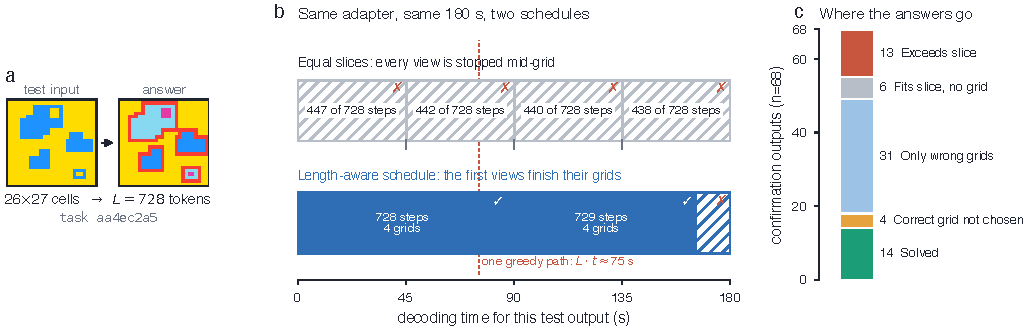
\includegraphics[width=\textwidth]{figures/teaser.pdf}
\caption{\textbf{A long answer runs out of time.} \textbf{a,} Task \texttt{aa4ec2a5} needs a $26\times27$ grid, 728 decoding steps. \textbf{b,} Decoding timelines from our pilot, same adapted model and budget. With equal slices (top), every view is stopped after about 440 steps; hatched blocks produced no candidate. The length-aware schedule (bottom) lets the first views finish, and the solver then submits the correct grid. \textbf{c,} Outcomes of the \ConfOutputs{} confirmation outputs under the reference selector. Only the bottom two segments can be improved by any selector; the red segment cannot be decoded in one slice at all.}
\label{fig:teaser}
\end{figure*}

\section{Related Work}
\paragraph{Test-time training for ARC.} Fine-tuning on the demonstrations of the task at hand was shown to work for ARC by \citet{akyurek2024} and in competition systems by \citet{cole2025}, who also vote over augmented predictions. \citet{li2024} combine transduction with program induction. \citet{franzen2025} introduced the DFS sampler and product-of-experts rescoring used by our solver; NVARC added large-scale synthetic data and frequency-aware rescoring \citep{sorokin2025}. Non-language-model approaches include tiny recursive networks \citep{jolicoeur2025}, compression without pretraining \citep{liao2025}, and vision transformers \citep{hu2025vision}. We do not propose a new model. We locate where a strong pipeline loses its answers and repair one cause.

\paragraph{Choosing among candidates.} Majority voting over samples \citep{wang2023} or augmentations \citep{cole2025} rewards answers that recur, while product-of-experts scoring aggregates likelihoods across views \citep{franzen2025}; NVARC mixes both \citep{sorokin2025}. We show that occurrence counts make rankings sensitive to duplicated records, and that removing this sensitivity does not raise accuracy when coverage is the binding constraint.

\paragraph{Decoding cost and test-time compute.} Speculative decoding reduces the number of sequential model calls \citep{leviathan2023}; the ARChitects built it into DFS during ARC Prize 2025 and reported a 4.3$\times$ runtime reduction \citep{franzen2025,architects2025}. The allocation of test-time compute has been studied for sampling and search \citep{snell2024}. Faster kernels and our schedule are complementary. Speed moves the line in Figure~\ref{fig:clock}; the schedule decides which outputs end up on the right side of it. Program-synthesis systems \citep{pourcel2025} face a related trade-off between program length and sampling budget.

\section{Approach}\label{sec:method}
\subsection{Solver}
Our base model is the NVARC Qwen3-4B checkpoint fine-tuned on ARC grids \citep{sorokin2025}. For each task, a rank-256 LoRA adapter \citep{hu2022} with rank-stabilized scaling \citep{kalajdzievski2023} is trained for 128 steps on 16 augmented copies of the demonstrations at learning rate $5\times10^{-5}$. Each test input is decoded under 16 views (eight geometric transforms, each with two colour permutations), grouped into four batches of four rows. The DFS keeps a prefix while its cumulative probability exceeds 0.2. Every distinct grid is rescored under eight augmentations, and the reference selector ranks grids by how often they were recorded and then by mean augmented negative log likelihood (NLL). Our in-competition entry reproduces the upstream notebook and its budget. For controlled studies and the post-deadline entries B0, S1, S2 and L1, we fix 360 seconds of decoding per task, divided equally among the task's view batches.

\subsection{Coverage and selection}\label{sec:decomp}
Let $P$ be the candidate pool for a test output with answer $y^\star$, and $S(P)$ the two submitted guesses. Then
\begin{equation}
\mathrm{pass@2}=\underbrace{\Pr[y^\star\in P]}_{\text{coverage}}\cdot\underbrace{\Pr[y^\star\in S(P)\mid y^\star\in P]}_{\text{selection}} .
\end{equation}
Our runs save every decoded grid with its view and all rescoring NLLs, so any selector can be replayed exactly. We compare the reference with seven alternatives that drop the occurrence term, normalize NLL by answer length, count the geometric views that support a grid, or pick a second guess that covers views the first one misses (Appendix~\ref{app:selectors}). Occurrence counts depend on how many times a grid happens to be recorded, which a deduplicating search can change without adding evidence. View-based scores do not:
\begin{proposition}[Record-copy invariance]\label{prop:copy}
Duplicating a record without changing its grid, view or scores leaves the view-support ranking and the joint coverage pair unchanged. A selector that keeps the reference's first answer inherits every change of that answer.
\end{proposition}
The proof follows because view support is a set and the per-view score a minimum (Appendix~\ref{app:selectors}). Stability, however, is not accuracy; Section~\ref{sec:selection} measures both.

\subsection{The decoding clock}\label{sec:clock}
\begin{figure*}[t]
\centering
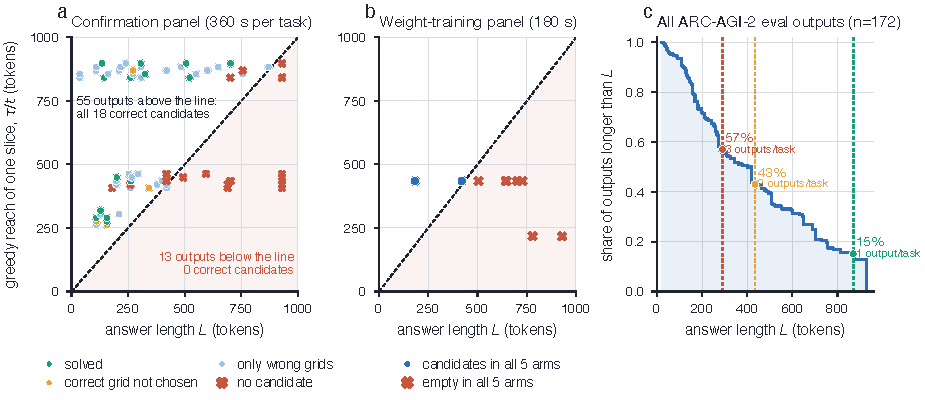
\includegraphics[width=\textwidth]{figures/clock.pdf}
\caption{\textbf{The decoding clock.} Greedy reach is the slice length divided by the measured time per forward pass (\StepMs\,ms). Outputs in the shaded region cannot finish even one greedy path within a slice. \textbf{a,} Confirmation outputs by outcome. \textbf{b,} The nine outputs of panel W, pooled over five training arms: the two outputs within reach have candidates in every arm, the seven beyond it in none. \textbf{c,} Answer lengths over all ARC-AGI-2 public evaluation outputs, with the greedy reach of a 360-second budget for tasks with one, two and three test outputs.}
\label{fig:clock}
\end{figure*}
Threshold DFS advances all rows of a batch in lockstep. Each model call extends every live prefix by one token, and a candidate is recorded only when its end token is expanded. A reply to an $h\times w$ grid has $hw$ cell tokens, $h-1$ row breaks and an end token, so $L=hw+h$.
\begin{proposition}[Reachability]\label{prop:reach}
If each model call takes at least $t$ seconds and a batch runs for $\tau$ seconds after a prefill of $p$ seconds, the batch can record a candidate of length $L$ only if $L\,t\le\tau-p$.
\end{proposition}
\begin{proof}
Recording the candidate requires expanding its $L$ tokens along one path, and each expansion needs the previous call's output, so the calls are sequential.
\end{proof}
\begin{corollary}\label{cor:slice}
If a budget $B$ is split equally among four batches for each of $m$ test outputs, every output with $L>(B/4m-p)/t$ has zero coverage, regardless of the model, the adapter, or the cutoff.
\end{corollary}
The bound is only a necessary condition, but it is computable before decoding and independent of model quality. We call $\rho=L\,t/\tau$ the \emph{load} of an output; outputs with $\rho>1$ are unreachable.

\subsection{Length-aware decoding}\label{sec:lengthaware}
Both changes leave the model, the cutoff and the scores untouched.

\paragraph{Exact iterative search.} The parent DFS recurses once per generated token and copies a full-vocabulary log-softmax to the host at every step. We replace recursion with an explicit stack and transfer only the 16 ARC-token columns. Rows still advance in lockstep, children are visited in the same stable order, and the deadline is tested at the same points. Against the verbatim parent code and a deterministic mock model, the iterative search returns identical suffixes, scores and forward-call counts in 120 complete and 80 deadline-truncated searches. Recursion depth equals answer length: a $30\times30$ reply needs 931 levels against CPython's default limit of 1{,}000 frames, and in our mock the recursive search fails beyond 993 tokens.

\paragraph{First-descent schedule.} Each test output receives an equal share $B/m$ of the task budget, tracked in a ledger, and its batches split what remains of that share. A batch may run past its slice only while it is still on its first greedy descent and no row has finished a candidate (Algorithm~\ref{alg:schedule}). The extension ends at the first finished candidate, the first backtrack, or when every row has been pruned.
\begin{proposition}[First-descent completion]\label{prop:ext}
If some row's greedy path in an output's first batch stays above the cutoff and $L\,t+p\le B/m$, the output receives a candidate. If the first batch records a candidate within its slice, the extension never triggers for that output.
\end{proposition}
\noindent The extension keeps descending until the candidate is recorded or the output's share is spent, which gives the first claim; the second holds by construction. Outputs that already succeed are therefore left alone. The ledger is a separate change that stops unused time from flowing between the outputs of one task.

\begin{algorithm}[t]
\caption{Length-aware view schedule for one task}\label{alg:schedule}
\small
\begin{algorithmic}[1]
\State $\textsc{left}[o]\gets B/m$ and $n[o]\gets 4$ for every test output $o$
\For{each view batch $b$ of output $o$, in parent order}
  \State \textbf{if} $\textsc{left}[o]\le 2$\,s \textbf{then} skip $b$
  \State $\tau\gets\textsc{left}[o]/n[o]$;\quad $T_{\max}\gets\textsc{left}[o]$
  \State Run iterative DFS on $b$ with deadline $\tau$; while on the first descent with no finished row, use deadline $T_{\max}$
  \State $\textsc{left}[o]\gets\textsc{left}[o]-\text{elapsed}$;\quad $n[o]\gets n[o]-1$
\EndFor
\end{algorithmic}
\end{algorithm}

\section{Results}
\ifpilot
\begin{figure*}[t]
\centering
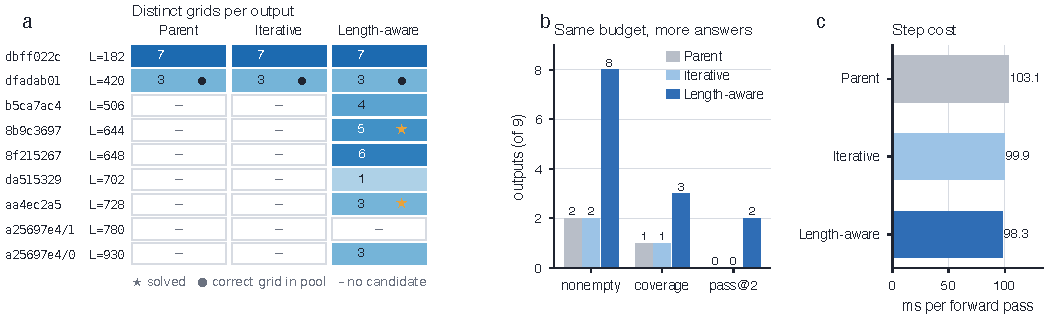
\includegraphics[width=\textwidth]{figures/pilot.pdf}
\caption{\textbf{Matched pilot on panel W} (one adapted model per task, 180\,s per arm). \textbf{a,} Distinct grids per output, rows ordered by answer length. The parent and iterative searches produce identical pools; the length-aware schedule decodes answers of up to \PilotMaxTokens{} tokens and solves two outputs that are empty under equal slices. \textbf{b,} Outputs with any candidate, with the correct candidate, and solved. \textbf{c,} Time per forward pass.}
\label{fig:pilot}
\end{figure*}
\fi
\subsection{Setup}
All experiments use the ARC-AGI-2 public evaluation set (\EvalTasks{} tasks, \EvalOutputs{} test outputs) on four NVIDIA L4 GPUs with internet disabled. Before any experiment, tasks were partitioned by a hash of their identifiers. The confirmation panel (\ConfTasks{} tasks, \ConfOutputs{} outputs) was decoded once, with all selectors fixed in advance. Panel W (8 development tasks, 9 outputs) hosts the training and decoding studies; arms share one adapted model per task wherever the comparison allows. Panel R (\SFourTasks{} fresh tasks, \SFourN{} outputs) hosts the spatial-repair study, and 32 reserve tasks were held back for a final confirmation. We report no training-set accuracy. The NVARC checkpoint may have seen public evaluation tasks during pretraining; our partition controls only our own development choices.

\begin{table}[t]\centering\footnotesize
\caption{Kaggle ARC-AGI-2 public leaderboard scores (percent of hidden test outputs). B0, S1, S2 and L1 share the generator, the 128-step adaptation and a 360-second decoding budget per task.}\label{tab:leaderboard}
\setlength{\tabcolsep}{3pt}\begin{tabular}{llr}\toprule
Entry & Status & Score \\\midrule
Upstream V1 \citep{rudra2026} & author & 33.89 \\
Our V1 reproduction & in comp. & 30.97 \\
B0: 360\,s decoding & late & 25.28 \\
S1: B0 + NLL-only selector & late & 22.78 \\
S2: B0 + anchored coverage & late & 23.61 \\
L1: B0 + length-aware decoding & late & 26.94 \\
\bottomrule\end{tabular}\end{table}


\subsection{Leaderboard}
Table~\ref{tab:leaderboard} lists the linked entries. Our reproduction of the upstream notebook scores 30.97, against 33.89 reported for the original. B0 caps decoding at 360 seconds per task and scores \ScoreBZero{}; this matched control is the reference for the post-deadline entries, each of which changes one component. Replacing the selector lowered the hidden-set score in both attempts, to \ScoreSOne{} (S1) and \ScoreSTwo{} (S2), consistent with the finding below that selection is not where answers are lost. L1 changes only decoding.

\begin{figure*}[t]
\centering
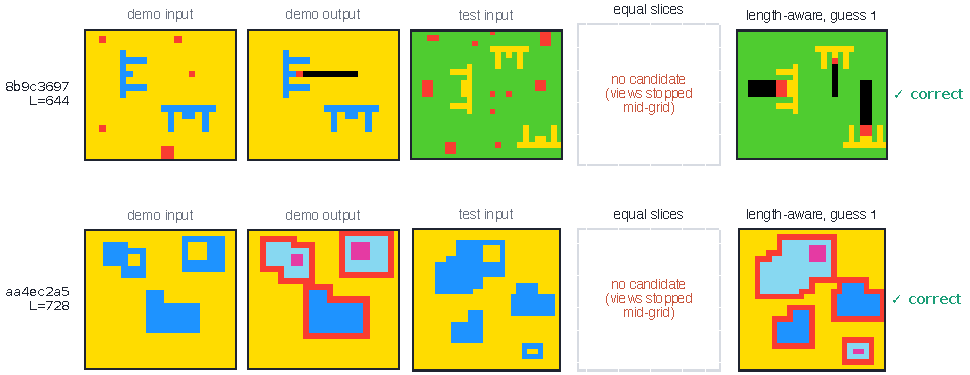
\includegraphics[width=\textwidth]{figures/gallery.pdf}
\caption{\textbf{The model needed time, not new knowledge.} The two outputs that only the length-aware schedule solves in the pilot. Each row shows the first demonstration, the test input, the outcome under equal slices, and the length-aware submission, which matches the answer cell for cell. Both answers are long (644 and 728 tokens), and the same adapted model produced both.}
\label{fig:gallery}
\end{figure*}
\subsection{Selection is near its ceiling}\label{sec:selection}
\begin{table}[t]\centering\footnotesize
\caption{Selection on frozen pools. Pass@1 and pass@2 count solved outputs out of 68 on the confirmation panel, whose pools contain 18 correct grids. The last column counts answer-set changes in 213 interventions that copy one development record eight times.}\label{tab:selectors}
\setlength{\tabcolsep}{4pt}\begin{tabular}{lccc}\toprule
Selector & Pass@1 & Pass@2 & Copy changes \\\midrule
Occurrence + NLL (reference) & 13 & 14 & 55 \\
NLL only & 11 & 14 & 0 \\
Token-normalized NLL & 11 & 14 & 0 \\
Geometric view support & 13 & 14 & 0 \\
Anchored view support & 13 & 14 & 48 \\
Anchored view union & 13 & 14 & 35 \\
Anchored soft coverage & 13 & 14 & 39 \\
Joint soft coverage & 13 & 14 & 0 \\
\bottomrule\end{tabular}\end{table}

On the confirmation panel, all eight selectors solve \ConfSolved{} of \ConfOutputs{} outputs (Table~\ref{tab:selectors}). Their first guesses differ, from 11 to 13 correct, but their pairs solve the same outputs, and the pools leave only \ConfMissed{} correct grids unselected. Copying records changes the reference's answer set in \CloneRef{} of \CloneTrials{} interventions, the view-based selectors' in none, and anchored coverage's in \CloneAnchor{} because it keeps the reference's first answer, exactly as Proposition~\ref{prop:copy} predicts. Selection is $\ConfSolved/\ConfOracle$ in Eq.~(1); coverage, at $\ConfOracle/\ConfOutputs$, is the factor that binds.

\subsection{The clock explains missing candidates}\label{sec:clockresults}
Our pilot logged every forward pass. On the \StepTasks{} tasks that finished no sequence, a four-row batch took a median of \StepMs\,ms per pass (range \StepLo--\StepHi\,ms). A 360-second task with one test output thus gives each batch 90\,s, about 870 passes; two and three outputs cut this to about 435 and 290.

Figure~\ref{fig:clock}a places each confirmation output against this reach. The \Unreach{} outputs below the line have no correct candidate between them, and \UnreachEmpty{} have no candidate at all. The \Reach{} outputs above the line hold all \ConfOracle{} correct candidates and all \ConfSolved{} solves. Being just above the line is not enough either: the \TightN{} outputs with load between 0.8 and 1 yield \TightEmpty{} empty pools and only \TightOracle{} correct candidate, because a batch that barely finishes one path has no time left to explore alternatives.

The effect is a property of the benchmark, not of our panel. \EvalOverPct\% of ARC-AGI-2 public evaluation answers are longer than 435 tokens (Figure~\ref{fig:clock}c). Under our budget and step time, \EvalUnreach{} of the \EvalOutputs{} outputs, in \EvalTasksUnreach{} of \EvalTasks{} tasks, cannot be decoded at all. Any solver that divides a wall-clock budget evenly across views or augmentations faces the same arithmetic with its own constants.

\subsection{Generator interventions under the clock}\label{sec:generator}
\begin{table}[t]\centering\footnotesize
\caption{Interventions on the generator. Panel W is the weight-training panel (8 tasks, 9 outputs; 2 of 9 outputs fit one view slice). Panel R is a fresh 24-task, 35-output repair panel. Coverage counts outputs whose pool contains the correct grid.}\label{tab:generator}
\setlength{\tabcolsep}{3.5pt}\begin{tabular}{lccc}\toprule
Arm & Panel & Pass@2 & Coverage \\\midrule
Original LoRA loss & W & 1/9 & 1/9 \\
Loss after first output (PoE) & W & 0/9 & 0/9 \\
Loss on final output only & W & 0/9 & 0/9 \\
Original loss, second run & W & 0/9 & 0/9 \\
Context-weighted loss & W & 0/9 & 0/9 \\
Parent search (backstop control) & W & 0/9 & 0/9 \\
Greedy completion backstop & W & 0/9 & 0/9 \\
\midrule
Full search, occurrence ranking & R & 4/35 & 7/35 \\
Shorter search, worst-view score & R & 5/35 & 7/35 \\
\quad + spatial repairs & R & 5/35 & 7/35 \\
\bottomrule\end{tabular}\end{table}

Table~\ref{tab:generator} collects our earlier attempts to improve the generator. On panel W we trained adapters that skip the first demonstration output, as in product-of-experts training \citep{franzen2025}, or that supervise only the final output; a second experiment reweighted outputs by the context available to them; a third reserved a fifth of each slice for a grammar-constrained greedy completion of empty streams. No arm solved more than one output. Figure~\ref{fig:clock}b shows why. Only \TrainReach{} of the \TrainN{} outputs fit a slice, and exactly those are nonempty in all five training arms. Whatever the objective, at most two outputs could change. The completion backstop makes the point most plainly: 129 of its 131 fallback streams hit the deadline, because a fifth of a slice that is already too short cannot finish a long grid.

On panel R, a spatial-repair arm raised pass@2 from \SFourBase{} to \SFourRepair{} of \SFourN. Replaying the same arm without repairs shows that worst-view scoring alone produced the extra solve; the \SFourRepairs{} evaluated repairs added no correct grid, and coverage stayed at \SFourOracle/\SFourN.

\subsection{Length-aware decoding}\label{sec:pilot}
The pilot repeats panel W with three arms that share one adapted model per task and receive 180 seconds each: the parent DFS, the iterative DFS with the same equal slices, and the iterative DFS with the length-aware schedule. Its predictions were frozen before launch: fewer empty pools than the 7/9 of every earlier arm, identical candidates for batches that finish before their deadline, and no slower forward passes.

All three held (Figure~\ref{fig:pilot}). The iterative search reproduced the parent's candidate sets on all \PilotEqN{} views that finished before their deadline in both arms, at \PilotMsIter\,ms per forward pass against \PilotMsParent\,ms. The length-aware schedule left \PilotEmptyLA{} of \PilotN{} outputs empty instead of \PilotEmptyCtl, finished \PilotFinLA{} sequences instead of \PilotFinCtl, raised coverage from \PilotCovCtl{} to \PilotCovLA{}, and solved \PilotSolvedLA{} outputs where the parent solved \PilotSolvedCtl, with \PilotLosses{} losses and a total time ratio of \PilotRatio. The two new solves, \texttt{8b9c3697} and \texttt{aa4ec2a5}, need 644 and 728 tokens; under equal slices their views were stopped after about 440 (Figure~\ref{fig:gallery}).

\ifconf
\begin{figure}[t]
\centering
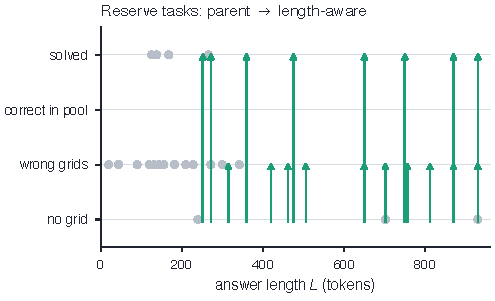
\includegraphics[width=\columnwidth]{figures/confirmation.pdf}
\caption{\textbf{Reserve-task confirmation.} Each arrow moves one output from its outcome under the parent search to its outcome under the length-aware schedule (green: better, red: worse); dots mark unchanged outputs.}
\label{fig:confirmation}
\end{figure}
The frozen configuration was then run once on the 32 reserve tasks (48 outputs), which no earlier experiment had touched (Figure~\ref{fig:confirmation}). Pass@2 is 5/48 for the parent search and 13/48 for the length-aware schedule, with 8 gains and 0 losses; the task-bootstrap 95\% interval for the difference is [6.0, 29.8] percentage points. Empty pools fall from 28 to 5, coverage moves from 5 to 13, and the total time ratio is 0.996. The gain observed on the development panel carries over to unseen tasks.

\else
The pilot met its promotion rule, and the frozen configuration is now being tested on the 32 reserve tasks, which no previous experiment has touched.
\fi
The linked entry L1 applies the schedule to the full hidden test set with B0's budget, adaptation and selector (Table~\ref{tab:leaderboard}).

\section{Discussion}
\paragraph{Why this matters for reaching 85\%.} Large outputs are common in ARC-AGI-2. A better model or a better ranking cannot help on an output the search never finishes, so a solver can keep improving on short tasks while its accuracy on long ones stays at zero. Two practices follow. First, report coverage by answer length, so that missing candidates are attributed to the right cause. Second, allocate time by length, either by decoding fewer views of long outputs or by letting one view finish before the next one starts. Faster decoding moves the line in Figure~\ref{fig:clock}; it does not remove it.

\paragraph{Beyond this solver.} Proposition~\ref{prop:reach} rests on two facts: candidates are produced token by token, and a batch has a deadline. It applies to any autoregressive grid decoder run under a wall-clock limit, whether it uses DFS, beam search or sampling, and to systems that write long programs. The coverage--selection replay needs only saved candidate pools.

\paragraph{Limitations.} Our panels are small, and panel W was reused across studies before the pilot. The step time comes from one run and varies with context length and hardware, which shifts the bound without removing it. Leaderboard scores are single executions. The pretrained checkpoint may overlap with public evaluation tasks.

\section{Conclusion}
A working test-time-trained ARC-AGI-2 solver loses most of its answers before selection begins: \ConfNoCorrect{} of \ConfOutputs{} held-out outputs never receive a correct candidate, and no selector we tried recovers any beyond the \ConfOracle{} that are present. A one-line bound on sequential decoding explains a large part of this gap, the null results of several training changes, and a property of the benchmark itself: under a common budget split, more than a quarter of ARC-AGI-2 evaluation outputs cannot be decoded at all. Letting each output finish its first greedy path recovers candidates that equal slicing destroys, at no extra cost. We release the search, the schedule, and the records needed to replay every number in this paper.

\paragraph{Code and data.} New code is released under MIT-0; the upstream notebook and model keep their Apache-2.0 attribution. Saved candidate pools, telemetry and analysis scripts reproduce every table and figure without a GPU.

{\small
\begin{thebibliography}{99}\setlength{\itemsep}{1pt}
\bibitem[Aky{\"u}rek et~al.(2024)]{akyurek2024} E.~Aky{\"u}rek, M.~Damani, L.~Qiu, H.~Guo, Y.~Kim, and J.~Andreas. The surprising effectiveness of test-time training for abstract reasoning. arXiv:2411.07279, 2024.
\bibitem[{The ARChitects}(2025)]{architects2025} The ARChitects. ARC Prize 2025 solution by the ARChitects: technical report. \url{https://lambdalabsml.github.io/ARC2025_Solution_by_the_ARChitects/}, 2025.
\bibitem[Chollet(2019)]{chollet2019} F.~Chollet. On the measure of intelligence. arXiv:1911.01547, 2019.
\bibitem[Chollet et~al.(2025)]{chollet2025} F.~Chollet, M.~Knoop, G.~Kamradt, B.~Landers, and H.~Pinkard. ARC-AGI-2: A new challenge for frontier AI reasoning systems. arXiv:2505.11831, 2025.
\bibitem[Cole and Osman(2025)]{cole2025} J.~Cole and M.~Osman. Don't throw the baby out with the bathwater: How and why deep learning for ARC. arXiv:2506.14276, 2025.
\bibitem[Franzen et~al.(2025)]{franzen2025} D.~Franzen, J.~Disselhoff, and D.~Hartmann. Product of experts with LLMs: Boosting performance on ARC is a matter of perspective. In \emph{ICML}, 2025. arXiv:2505.07859.
\bibitem[Hu et~al.(2022)]{hu2022} E.~J.~Hu, Y.~Shen, P.~Wallis, Z.~Allen-Zhu, Y.~Li, S.~Wang, L.~Wang, and W.~Chen. LoRA: Low-rank adaptation of large language models. In \emph{ICLR}, 2022.
\bibitem[Hu et~al.(2025)]{hu2025vision} K.~Hu et~al. ARC is a vision problem! arXiv:2511.14761, 2025.
\bibitem[Jolicoeur-Martineau(2025)]{jolicoeur2025} A.~Jolicoeur-Martineau. Less is more: Recursive reasoning with tiny networks. arXiv:2510.04871, 2025.
\bibitem[Kalajdzievski(2023)]{kalajdzievski2023} D.~Kalajdzievski. A rank stabilization scaling factor for fine-tuning with LoRA. arXiv:2312.03732, 2023.
\bibitem[Leviathan et~al.(2023)]{leviathan2023} Y.~Leviathan, M.~Kalman, and Y.~Matias. Fast inference from transformers via speculative decoding. In \emph{ICML}, 2023.
\bibitem[Li et~al.(2024)]{li2024} W.-D.~Li, K.~Hu, C.~Larsen, et~al. Combining induction and transduction for abstract reasoning. arXiv:2411.02272, 2024.
\bibitem[Liao and Gu(2025)]{liao2025} I.~Liao and A.~Gu. ARC-AGI without pretraining. Technical report, 2025.
\bibitem[Pourcel et~al.(2025)]{pourcel2025} J.~Pourcel, C.~Colas, and P.-Y.~Oudeyer. Self-improving language models for evolutionary program synthesis: A case study on ARC-AGI. In \emph{ICML}, 2025. arXiv:2507.14172.
\bibitem[Rudra(2026)]{rudra2026} K.~Rudra. Failed in AIMO, notebook version 1. Kaggle, \url{https://www.kaggle.com/code/koushikrudra/failed-in-aimo?scriptVersionId=312063593}, 2026.
\bibitem[Snell et~al.(2024)]{snell2024} C.~Snell, J.~Lee, K.~Xu, and A.~Kumar. Scaling LLM test-time compute optimally can be more effective than scaling model parameters. arXiv:2408.03314, 2024.
\bibitem[Sorokin and Puget(2025)]{sorokin2025} I.~Sorokin and J.-F.~Puget. NVARC solution to ARC-AGI-2 2025. Technical report, 2025.
\bibitem[Wang et~al.(2023)]{wang2023} X.~Wang, J.~Wei, D.~Schuurmans, Q.~Le, E.~Chi, S.~Narang, A.~Chowdhery, and D.~Zhou. Self-consistency improves chain of thought reasoning in language models. In \emph{ICLR}, 2023.
\end{thebibliography}
}

\clearpage
\appendix
\section{Selectors and proofs}\label{app:selectors}
Let $R$ be the multiset of records for one test output. Record $r$ holds a grid $y_r$, its generating geometric view $v_r\in D_4$, and augmented NLLs $L_{rj}$ with answer-token counts $t_{rj}$, $j=1,\dots,m_r$.

\paragraph{Reference.} Distinct grids are ranked by decreasing $B(y)=n_y-n_y^{-1}\sum_{r:y_r=y} m_r^{-1}\sum_j L_{rj}$, where $n_y$ is the number of records of $y$, as in the upstream code. Because NLLs are small, the count $n_y$ dominates. The NLL-only ablation removes the count; the token-normalized ablation divides each $L_{rj}$ by $t_{rj}$.

\paragraph{View support.} For each grid and view, $\ell_v(y)=\min_{r:y_r=y,v_r=v} m_r^{-1}\sum_j L_{rj}/t_{rj}$ and $V_y=\{v:\exists r,\,y_r=y,\,v_r=v\}$. The view-support selector maximizes $|V_y|$ and breaks ties by the mean of $\ell_v(y)$. The anchored variant keeps the reference's first answer and picks the best other grid supported by at least two views.

\paragraph{Coverage.} With $q_v(y)\propto\exp(-\ell_v(y))$ normalized over grids observed in view $v$, a pair $S$ has coverage $F(S)=|V|^{-1}\sum_v\max_{y\in S}q_v(y)$. The joint selector maximizes $F$ over pairs; the anchored selector fixes the first answer.

\paragraph{Proof of Proposition~\ref{prop:copy}.} Copying a record changes neither the set $V_y$ nor any minimum $\ell_v(y)$, hence neither the support ranking nor $q_v$ or $F$. Tie rules depend only on grids. If the reference's first answer changes, any selector whose first component equals it changes too.

\section{Panels and protocols}\label{app:protocol}
\paragraph{Confirmation.} 48 tasks, 68 outputs, 128 adaptation steps, 360\,s decoding per task, selectors fixed before decoding. Bootstrap intervals resample whole tasks.
\paragraph{Panel W.} From the 12-task development panel, tasks with at least three demonstrations, then the eight smallest by demonstration cells. All arms complete 128 steps; arm order rotates over permutations. Training arms received identical augmented inputs; supervised-token counts and parameter changes were verified per arm.
\paragraph{Panel R.} 24 fresh tasks, 35 outputs. The control decodes for 360\,s; the repair arm decodes for 270\,s and scores repairs for 90\,s with the same adapted model.
\paragraph{Pilot and reserve confirmation.} Panel W (pilot) and the 32 reserve tasks (confirmation); 180\,s per arm, one shared adapted model per task, arm order rotated, protocol and predictions frozen before launch.
\paragraph{Linked entries.} B0, S1, S2 and L1 process every hidden task with 128 adaptation steps and 360\,s of decoding per task. Before submission, each version ran on four public tasks, and its candidates and selections were replayed locally.

\section{Reproducibility}
Each GPU run stores the pinned notebook and its source hash, per-task telemetry, all candidate pools, and post-hoc metrics computed only after predictions were frozen. Local scripts check that replayed selections and metrics match the cloud outputs before any number enters the paper, and a single script regenerates every table and figure from these records.
\end{document}
